\documentclass{acm}
\usepackage[dutch]{babel}

\begin{document}

\title{User Experience Design}
\subtitle{Muziektafel}

\numberofauthors{5}
\author{
\alignauthor Robert Dahmen\\
       \affaddr{Universiteit Twente}\\
       \email{r.j.dahmen@ \\ student.utwente.nl}
\alignauthor Alexander Drechsel
       \affaddr{Universiteit Twente}\\
       \email{alexander\_drechsel3@ \\ hotmail.com}
\and
\alignauthor Niels Kamp\\
       \affaddr{Universiteit Twente}\\
       \email{niels.kamp@xs4all.nl}
\alignauthor Kasper Vaessen\\
       \affaddr{Universiteit Twente}\\
       \email{k.m.vaessen@ \\ student.utwente.nl}
\alignauthor Niels Visser\\
       \affaddr{Universiteit Twente}\\
       \email{nsvisser@gmail.com}
}
\maketitle

\begin{abstract}
Samenvatting.
\end{abstract}

\keywords{multi-touch, table, inexperienced user}

\section{Introductie}
Multi-touch interfaces zijn de laatste jaren steeds meer onderdeel geworden van het dagelijks leven; smartphones, tablets hebben hier allemaal ondersteuning voor en maken levendig gebruik van de mogelijkheden die multi-touch biedt. Maar naast deze apparaten die steeds meer mensen bij zich hebben, zijn er ook ontwikkelingen op multi-touch gebied voor apparaten met grotere schermen. Denk hierbij aan computermonitoren, televisies en zogenaamde video walls: de technologische ontwikkeling richt zich op multi-touch.

Zo ook bij opdrachtgever KITT Engineering, waar men tracht een brug te slaan tussen creatieve idee\"en en de uiteindelijke toepassing daarvan. KITT heeft in-house een multi-touch tafel ontwikkeld, waarmee het de mogelijke toepassingen van grote multi-touch oppervlakken wil onderzoeken. Ook wil men bekijken hoe de bedachte technologie in de echte wereld gebruikt kan worden en hoe mensen reageren op dergelijke technologie wanneer ze ermee in aanraking komen.

\subsection{Opdrachtsomschrijving}
De opdracht bestaat uit het ontwikkelen van een applicatie die de mogelijkheden van multi-touch ten volle benut en mensen op een intu\"itieve manier kennis laat maken met het fenomeen van een multi-touch interface ter grootte van een tafel. De applicatie moet mensen zowel uitnodigen om zelfstandig uit te proberen wat een multi-touch tafel kan als de mogelijkheid bieden om gezamenlijk te werken aan het cre\"eren van iets moois.

Hoe aan deze opdracht invulling gegeven moet worden, is niet gespecificeerd. Het is aan de projectgroep om deze invulling te bedenken en de opdrachtgever ten behoeve van sturing bij het ontwerpproces te betrekken.

\subsection{Inhoud}
In dit paper wordt in hoofdstuk~\ref{sec_domein} ingegaan op het domein van de te realiseren applicatie: door wie zal het eindresultaat gebruikt worden en met welk doel. Ook wordt beschreven aan welke functionele eisen de gerealiseerde applicatie moet voldoen om de doelgroep succesvol dit doel te laten bereiken. In hoofdstuk~\ref{sec_concept} staat beschreven hoe deze functionele eisen verwerkt zijn in meerdere conceptuele ontwerpen, welke inspiratiebronnen zijn gebruikt voor de bedachte concepten en welk van deze ontwerpen vervolgens in samenspraak met de opdrachtgever is uitgekozen om verder uit te werken. Dit verder uitwerken wordt gedaan in hoofdstuk~\ref{sec_detail}. In dit hoofdstuk staat een functionele specificatie van het gekozen ontwerp en een beschrijving van de technische realisatie: een technisch ontwerp.

Na het ontwerpen en realiseren van de applicatie, zal de usability ervan getest moeten worden, alsook de user experience. De opzet van deze tests en de resultaten ervan staan beschreven in hoofdstuk~\ref{sec_evaluatie}. Naar aanleiding van deze resultaten zal in hoofdstuk~\ref{sec_discussie} behandeld worden in hoeverre de gerealiseerde applicatie voldoet aan de eerder gestelde eisen.

Tot slot volgt in hoofdstuk~\ref{sec_conclusie} een reflectie van het doorlopen ontwerpproces, het eindresultaat en eventuele verbeterpunten.

\section{Domein}
\label{sec_domein}
Een multi-touch tafel is een experimentele techniek die nog niet breed toegepast wordt in de wereld. Het wordt meestal voor specialistische toepassingen gebruikt, zoals het bedrijfsleven, en in state-of-the-art producten, die bedoeld zijn om de mogelijke toepassingen te onderzoeken -- zoals het gebruik in musea om te kijken of kinderen met een interactief systeem meer opsteken van hun bezoek of hun bezoek positiever beoordelen.

Het concept multi-touch is met de sterke opkomst van multi-touch capable smartphones en tablets echter niet meer uit de hedendaagse wereld weg te denken. Wel is het zo dat de adoptie van deze apparaten voornamelijk in de jongere demografen een groeispurt doormaakt, terwijl de ouderen van dagen hier minder in meegaan. Aangezien het doel van de tafel is om iedereen, jong en oud, kennis te laten maken met het concept van een multi-touch tafel, is het van belang om bij het ontwerp rekening te houden met de intu\"itiviteit van het gebruik ervan: iedereen moet ermee kunnen werken. Eventueel na een korte instructie, maar bij voorkeur zonder.

Vanwege het open karakter van de opdracht -- het mensen laten kennismaken met het concept multi-touch tafel door middel van een applicatie die uitnodigt tot gebruik -- zijn de functionele eisen in deze fase beperkt. Vanwege de brede doelgroep en de ongelijke ervaring van deze doelgroep met multi-touch interfaces, worden er vooral eisen gesteld aan de usability van de applicatie: hiermee worden de eisen bedoeld die invloed hebben hoe gebruikers de applicatie gebruiken en wat de gewenste ervaring van het gebruik is en niet de precieze werking van het te bouwen concept. Hieronder volgt een opsomming van deze eisen met argumentatie.

\begin{itemize}
	\item \textbf{Het doel en de wijze van gebruik van de muziektafel moet voor gebruikers op het eerste oog duidelijk zijn.} \\ Om mensen uit te nodigen de applicatie te gebruiken moet deze simpel in gebruik zijn en een vlakke leercurve hebben.
	\item \textbf{De muziektafel moet door 1 tot minstens 4 gebruikers te gebruiken zijn.} \\ Mensen kunnen er voor kiezen om met zijn vieren te beginnen met de applicatie, maar het moet ook mogelijk zijn om met minder te beginnen en voor mensen om zich later erbij aan te sluiten. Voor deze latere aansluiters helpt het om te zien dat andere mensen reeds bezig zijn met de tafel. Zo kunnen zij er zonder druk bij gaan staan en in hun eigen tempo de applicatie leren besturen, zonder dat zij andere spelers ophouden.
	\item \textbf{Het getoonde speelveld moet opgedeeld zijn in vier (4) gedeelten.} \\ Om mensen uit te nodigen mee te doen, zijn er te allen tijde vier speelvelden zichtbaar. Deze worden niet gebruikt indien er minder dan vier spelers zijn (tenzij \'e\'en speler meerdere speelvelden bedient), waardoor mensen zich eenvoudig in de spelbeleving kunnen mengen, zonder verdere stappen te moeten nemen.
	\item \textbf{Iedere speler heeft een eigen gedeelte van het speelveld tot zijn beschikking.} \\ Om ervoor te zorgen dat spelers elkaar niet in de weg zitten en iedereen op zijn eigen tempo kan werken met de applicatie, heeft iedere speler een eigen speelveld.
\end{itemize}

\section{Conceptueel Ontwerp}
\label{sec_concept}
In aanloop naar het ontwerp heeft de opdrachtgever vier voorstellen gekregen, verdeeld over twee categorie\"en: \'e\'en co\"operatief en drie competitief. Uit deze voorstellen is uiteindelijk een concept gekozen dat het beste aansloot bij het gedachtegoed van de opdrachtgever en het doel dat de opdrachtgever met de applicatie voor ogen had.

Het co\"operatieve voorstel bestond uit een muziektafel waarbij meerdere mensen samen werkten aan het componeren van een harmonieuze symfonie. Dit concept is geïnspireerd op een muziekspelletje op internet, waarbij met verschillende instrumenten een symfonie gecreëerd kan worden [http://games.co.za/music-sequencer.html]. De drie competitieve voorstellen waren spellen. De eerste was een boogschietspel, waarbij iedere speler moest voorkomen dat zijn doelwit geraakt werd door de pijlen van andere spelers af te weren, terwijl hij probeerde de doelwitten van de andere spelers te raken. De populariteit van spellen als Angry Birds [http://www.angrybirds.com/] diende hierbij ter inspiratie voor het mikken: de pijl en boog vormden hier een invulling van. Een ander voorstel was een multiplayer snake waarbij spelers elkaars slang moesten ontwijken, terwijl ze streefden naar het opeten van punten en bonussen. Ten slotte was er nog een voetbaltafel waarbij twee teams proberen de bal in het doel van het andere team te krijgen door middel van knoppen langs de zijkant die de poppetjes van hun team op het speelveld aansturen.

Vanwege het korte tijdsschema van dit project zijn deze voorstellen alleen kort, tekstueel uitgewerkt en voorzien van een ruwe schets. Er zijn geen functionele requirements voor elk voorstel opgesteld. De voorstellen zijn met een mondelinge toelichting overgedragen aan de opdrachtgever en uiteindelijk is in overleg besloten te kiezen voor de muziektafel. Dit concept had voor nieuwe gebruikers de laagste instapdrempel, liet het best de mogelijkheden van de multi-touch tafel zien en bevat een creatieve draai, waar de opdrachtgever in zijn missie naar streeft. [FIXME: motivatie]

\subsection{Eisen Muziektafel}
Voordat begonnen kon worden aan het functionele ontwerp van de muziektafel, moet eerst uitgezocht worden aan welke functionele eisen dit ontwerp zal moeten voldoen. Hieronder volgende de functionele eisen, waaraan het ontwerp, in combinatie met de geformuleerde eisen uit hoofdstuk~\ref{sec_domein}, moet voldoen. Indien een eis toelichting vereist, is deze gegeven, alsmede van wie de eis afkomstig is.

\begin{itemize}
	\item \textbf{Met ieder speelveld wordt een (1) muziekinstrument bespeeld.} \\ Door deze eis kunnen spelers doen waar zij het meeste zin in hebben, zonder gehinderd te zijn door het instrument dat andere spelers willen bespelen.
	\item \textbf{Een speler kan zelf kiezen welk instrument hij bedient met zijn speelveld.} \\ Dankzij deze eis kan iedere speler het voor hem meest interessante instrument bespelen, wat mensen met tal van verschillende, muzikale interesses uitnodigt gebruik te maken van de multi-touch tafel.
	\item \textbf{Een speler kan zelf bepalen met welk volume zijn instrument afgespeeld wordt.} \\ Om te voorkomen dat een speler afbraak doet aan de gecreëerde melodie, is het wenselijk als hij in dat geval het volume van zijn muziekinstrument kan aanpassen. Op deze wijze kan hij nog steeds spelen met de multi-touch tafel, zonder het idee te hebben andere spelers lastig te vallen. Deze eis volgt uit de wens om de tafel voor veel mensen, van iedere leeftijd, toegankelijk te maken.
	\item \textbf{Elk speelveld vertegenwoordigt één instrument. Door de aanraak-interface kunnen mensen bepalen van welk instrument op welk moment welke tonen afgespeeld worden.} \\ Deze eis volgt uit de wens van de opdrachtgever: spelers moet kennis maken met de multi-touch tafel.
	\item \textbf{De spelers moeten tegelijkertijd met minstens een (1) aanraking per speler tegelijk input kunnen geven aan de af te spelen noten.} \\ Ook deze eis volgt uit de wens van de opdrachtgever om de eigenschappen van de multi-touch tafel te etaleren: spelers moeten hun eigen speelveld kunnen bedienen, zonder dat de limieten van de tafel ze daarbij hindert. [FIXME: reference: The cueTable: Cooperative and Competitive Multi-Touch Interaction on a Tabletop]
	\item \textbf{De noten van de vier muziekinstrumenten worden gecombineerd tot een harmonieuze melodie.} \\ Deze eis volgt uit de wens van de opdrachtgever om mensen aan te zetten tot het gebruik: des te meer mensen meehelpen aan het componeren van een melodie, des te beter deze wordt.
	\item \textbf{Het mag niet mogelijk zijn dat er een valse melodie gecreëerd wordt.} \\ Als de gecomineerde melodie prettig in het gehoor ligt, zijn gebruikers sneller geneigd om door te gaan met het componeren ervan. [citation needed]
	\item \textbf{De af te spelen noten zijn per 16e maat in te stellen.} \\ De noten zijn per 16e maat instelbaar. Het is nog onduidelijk wat voor het componeren van muziek uiteindelijk wenselijker is: indien een noot twee 16e maten achter elkaar aanstaan, wordt deze dan gedurende deze twee 16e maten continu afgespeeld, of wordt de noot de tweede 16e maat opnieuw aangeslagen.
	\item \textbf{Per 16e maat zijn nul of meer noten te selecteren die afgespeeld moeten worden.} \\ Hierdoor is het mogelijk om per muziekinstrument zowel harmonie als melodie te krijgen.
	\item \textbf{Per muziekinstrument kunnen tien (10) toonhoogten en 16 16e maten geselecteerd worden.} \\ Deze eis volgt uit het niet mogen componeren van een valse melodie. Door per octaaf de noten \textit{A, B, D, E en F\#} te gebruiken, kan geen valse melodie gecreëerd worden. [citation needed] Om ervaren gebruikers de mogelijkheid te geven om complexere melodie\"en te componeren, hebben ze de beschikking over twee octaven.
	\item \textbf{Als er langer dan een minuut geen gebruik wordt gemaakt van het programma, wordt een demomodus afgespeeld, waarbij een voorgeprogrammeerde melodie wordt opgebouwd en afgespeeld. Zodra een speler het scherm aanraakt, wordt of de eerder gebouwde melodie op ieders speelveld teruggezet of wordt een leeg speelveld getoond.} \\ Deze eis volgt uit de wens om de applicatie uitnodigend te maken. Door deze demo-modus wordt voor de gebruiker gedemonstreerd wat er met de applicatie kan en hoe deze met behulp van de multi-touch tafel bediend kan worden.
	\item \textbf{De muziek wordt standaard afgespeeld met een snelheid van 120 beats per minuut (BPM), wanneer dit niet instelbaar is.} \\ Deze eis zorgt ervoor dat er een redelijke tempo in de muziek zit, zodat een simpele gecre\"eerde melodie al spannend genoeg is om aan verder te werken. [citation needed]
	\item \textbf{Tijdens het afspelen wordt de gecreëerde muziek gevisualiseerd.} \\ Dit is wederom voor het uitnodigende karakter van de applicatie gedaan, om naast de ge\"interesseerden in audio ook de visueel ingestelde mensen aan te trekken.
	\item \textbf{Nadat de laatste kwartmaat afgespeeld is, wordt opnieuw begonnen bij de eerste kwartmaat.} \\ Om te voorkomen dat spelers steeds de melodie opnieuw moeten starten en om de bediening zo eenvoudig mogelijk te houden, is het afspelen van de melodie een doorlopend proces: men kan zo aanschuiven, de noten van zijn instrument instellen en meteen het resultaat horen.
	\item \textbf{De door de spelers geselecteerde noten blijven geselecteerd wanneer opnieuw bij de eerste kwartmaat begonnen wordt.} \\ Ook dit is onderdeel van de tafel uitnodigend maken en spelers het idee te geven dat ze iets aan het bouwen zijn: hun melodie blijft bestaan en verbeterd worden.
	\item \textbf{Het speelveld van een speler moet door de speler in \'e\'en handeling ontdaan kunnen worden van alle geselecteerde noten.}
\end{itemize}

\subsection{Uitwerking Muziektafel}
\subsubsection{Eerste ontwerp}

Op basis van deze eisen is een eerste conceptueel ontwerp gemaakt. De schets van dit ontwerp is opgenomen in Figuur~\ref{fig:muziektafel_v1}. Te zien hierin is allereerst de cirkel waarop spelers noten kunnen selecteren: de notenbalk. Het onderscheid tussen de verschillende speelvelden is aangegeven door vier verschillende kleuren. Op de cirkel liggen 10 toonhoogtes en 16 16e maten. Standaard is het tempo ingesteld op 120 beats per minuut, maar dit is door middel van de plus- en minknop in het midden van de cirkel in te stellen.

Onder ieder speelveld staan twee knoppen; een waarmee de geselecteerde noten van het speelveld verwijderd kunnen worden en een waarmee een instrument gekozen kan worden. Om aan te geven dat de linkerknop knop iets verwijderd, is gebruik gemaakt van een vuilnisbak-icoon. Met de rechterknop hebben spelers de kans om het instrument van hun speelveld aan te passen. Om aan te geven dat het hun instrumentkeuze betreft, wordt er op de knop een icoon getoond van het instrument waar ze momenteel mee spelen. De knoppen hebben dezelfde kleur als het speelveld, om voor spelers duidelijk te maken welke knoppen bij hun gedeelte van de cirkel horen. Wanneer op de instrumentkeuzeknop gedrukt wordt, wordt er een overlay getoond over de notenbalk. In deze overlay kan de speler een van de acht beschikbare instrumenten kiezen: een piano, gitaar, basgitaar, drumstel, fluit, viool, orchel of triangel. In Figuur~\ref{fig:muziektafel_v1} is deze overlay voor het blauwe speelveld zichtbaar. Wanneer de speler op een instrument klikt, sluit de overlay zich en zal de notenbalk van dat speelveld afgespeeld worden met het gekozen instrument.

Daarnaast is er boven de notenbalk een extra onderdeel zichtbaar: de alternatieve notenbalk. Iedere speler heeft de beschikking over 2 sets van 16 16e maten. Een van deze twee wordt weergegeven op de notenbalk en kan door de speler bewerkt worden, de ander wordt boven de notenbalk weergegeven als knop. Wanneer op die knop gedrukt wordt, worden de twee sets noten omgewisseld; de set noten van de notenbalk wordt vervangen door de andere set. Bij het afspelen van de noten wordt vanaf de eerstvolgende 16e maat de nieuwe set noten gebruikt. Wanneer de wis-knop linksonder op het speelveld gebruikt wordt, wordt alleen de set noten gewist die op dat moment in de notenbalk staat. De andere set blijft bewaard.

\begin{figure}
  \includegraphics[width=84mm]{img/muziektafel_v1}
  \caption{Schets van het eerste ontwerp}
  \label{fig:muziektafel_v1}
\end{figure}

Zodra de applicatie gestart wordt, wordt begonnen met het afspelen van de notenbalk. De noten van de vier speelvelden worden per 16e maat tegelijk afgespeeld. Om aan te geven welke 16e maat afgespeeld wordt, wordt de notenbalk voor deze 16e maat gearceerd. In Figuur~\ref{fig:muziektafel_v1} is dat te zien aan de feller gekleurde kolommen.

\subsubsection{Tweede ontwerp}
Nog voor de evaluatie met eindgebruikers van het initiële ontwerp werden in samenspraak met de opdrachtgever echter verscheidene gebreken geconstateerd. Het eerste dat opviel, was de drukte van de interface: elk gedeelte van het speelveld wordt gebruikt voor een of andere functionaliteit. De oorspronkelijk bedachte visualisatie op de achtergrond van de speelvelden - bedoeld om de muziektafel naast het oor ook voor het oog uitnodigend te laten zijn - krijgt hierdoor erg weinig ruimte. Ook zou die visualisatie de interface nog drukker maken. Een ander punt dat de bruikbaarheid van de applicatie niet ten goede komt, is dat het door de cirkelvormigheid van de notenbalk moeilijk te zien is welke noten op dezelfde rij zitten. Dit bemoeilijkt het kunnen zien van de verschillende toonhoogtes binnen de 16 16e maten en daarmee het eenvoudig componeren van de gewenste melodie.

\begin{figure}
  \includegraphics[width=84mm]{img/muziektafel_v2}
  \caption{Schets van het tweede ontwerp}
  \label{fig:muziektafel_v2}
\end{figure}

De gekozen kleurstelling bleek daarnaast niet geschikt voor kleurenblinden: de aangrenzende speelvelden zijn voor hen niet goed te onderscheiden. Ook werd de alternatieve notenbalk niet intuïtief genoeg bevonden, terwijl deze wel een aanzienlijk deel van de interface in beslag nam.

Naar aanleiding van deze interne bezwaren tegen het ontwerp, is besloten om het ontwerp grondig aan te passen. Bepaalde functionaliteit is geschrapt of uit de primaire interface gehaald en achter een menu geplaatst; de primaire interface is versimpeld zodat er standaard niet meer in beeld is dan nodig. Het resultaat van dit herontwerp is te zien in Figuur~\ref{fig:muziektafel_v2}. De grote knoppen uit het eerste ontwerp zijn gecondenseerd naar twee kleinere knoppen boven de notenbalk. De eerder aanwezige alternatieve notenbalk is geschrapt (FIXME: of verplaatst naar een submenu) en het instellen van tempo heeft niet langer de centrale rol tussen de speelvelden en ook de knop voor het leeggooien van de notenbalk is verwijderd. Deze drie opties zijn in plaats daarvan achter de instellingenknop geplaatst. Deze knop heeft een tandwiel als icoon, waarvan het gebruik als instellingen-icoon als ingeburgerd wordt verondersteld.

De verwijdering van al deze knoppen heeft ervoor gezorgd dat de interface opgeruimder oogt, terwijl de visualisatie meer ruimte heeft gekregen. Door de speelvelden niet langer doorzichtig te maken worden deze beter onderscheidbaar van de visualisatie, terwijl de opvallender kleuren bijdragen aan het aantrekkelijk maken van het ontwerp. Daarbij zijn de kleuren nu zo gekozen zijn dat de speelvelden voor kleurenblinden goed te onderscheiden zijn en zijn de verschillende toonhoogtes om en om anders gekleurd zodat deze beter van elkaar te onderscheiden zijn.

\subsection{Evaluatie LoFi-prototype}
\subsubsection{Opzet}
Om uit te vinden hoe intuïtief het bedachte ontwerp voor de gewenste doelgroep is, is de schets van het tweede ontwerp voorgelegd aan een aantal proefpersonen. Ook is een eerste versie van de applicatie gemaakt, die alleen een werkende notenbalk-cirkel bevat. Door middel van de muis kunnen noten aangeklikt worden welke afgespeeld zullen worden door vier voorgeprogammeerde instrumenten: een voor ieder speelveld. De applicatie kan hiermee gebruikt worden door één persoon.

Vanwege het gewenste uitnodigende karakter van de multi-touch tafel is gekozen om bij de evaluatie voornamelijk de intuïtieve werking van het ontwerp te testen. We hebben hierbij het volgende script gebruikt om de gebruikers te ondervragen:

\begin{itemize}
  \item De proefpersoon krijgt de schets van het ontwerp uit Figuur~\ref{fig:muziektafel_v1} te zien.
  \item \textbf{Vraag 1:} Als je naar de interface kijkt, wat denk je dat de applicatie doet?
  \item \textbf{Vraag 2:} Hoe zou je deze besturen? Wat zou je als eerste proberen?
  \item Na deze twee vragen wordt de proefpersoon uitgelegd dat het een muziekapplicatie betreft.
  \item \textbf{Vraag 3:} Nu je weet wat de applicatie doet, hoe zou je het besturen?
  \item \textbf{Vraag 4:} Voor hoeveel spelers is het spel geschikt?
  \item Indien de speler niet bedacht heeft dat het een multi-touch applicatie is, wordt hem de besturing van de notenbalk uitgelegd. Ook wordt er verteld dat het op een multi-touch tafel gespeeld wordt samen met anderen.
  \item \textbf{Vraag 5:} Vind je de representatie van noten duidelijk?
  \item \textbf{Vraag 6:} Als je het muziekinstrument wilt veranderen, hoe zou je dat doen?
  \item \textbf{Vraag 7:} Als je het tempo van de muziek wilt aanpassen, hoe zou je dat doen?
  \item \textbf{Vraag 8:} Waar denk je dat de knop met de muzieknoot voor dient?
  \item \textbf{Vraag 9:} Als je opnieuw wilt beginnen met een leeg veld, hoe zou je dat doen?
  \item \textbf{Vraag 10:} Waar denk je dat de knop met het tandwiel voor dient?
  \item \textbf{Vraag 11:} Heb je verder nog opmerkingen over het doel van de applicatie en hoe de interface er nu uit ziet?
\end{itemize}

De eerste twee vragen dienen om te achterhalen of de applicatie de juiste indruk geeft bij mensen: nodigt de applicatie uit tot muziek maken? De derde en vierde vraag zijn bedoeld om te controleren of de interface laat zien het door meerdere mensen tegelijk bestuurd kan worden en of hoe de proefpersoon zelf denkt dat dit werkt. Vervolgens worden een voor een naar de intuïtiviteit van de overige features gevraagd en gecontroleerd of de gebruikte iconen begrepen werden. Indien de proefpersoon het antwoord op een vraag niet wist, werd hem dit na vraag 2 en 4 uitgelegd, aangezien dit noodzakelijk was voor het vervolg van de evaluatie. Bij de andere vragen werd deze uitleg zoveel mogelijk voorkomen om de proefpersoon niet te beïnvloeden. Bij de laatste vraag kon de gebruiker alle feedback die hij verder nog had kwijt.

\subsubsection{Resultaten LoFi-evaluatie}
Aangezien de doelgroep van de applicatie breed is, is bij de evaluatie geprobeerd om deze groep van geïnterviewden zo breed mogelijk te houden. Onder de ondervraagden zitten studenten, mensen van middelbare leeftijd en senioren. Van de proefpersonen begreep het merendeel na de eerste oogopslag dat het muziek een rol speelt bij de applicatie; het muzieknoot-icoon heeft aan dit besef bijgedragen. Ook was het de meeste mensen duidelijk dat de applicatie bestuurd kon worden door op de notenbalk te klikken. Een enkeling zou eerst op het de instrumentenkeuzeknop klikken, maar alle proefpersonen zouden in ieder geval ergens in de interface klikken - ook zonder uitleg.

Minder duidelijk was het dat het een applicatie voor vier spelers betrof. De kleuren werden als onderscheiding van verschillende instrumenten aangemerkt en niet als onderscheiding van speelvelden voor verschillende spelers. Enkelen zagen wel in dat het met meerdere mensen gespeeld kon worden, maar achtten het primair voor één speler vanwege deze verwarde scheiding van speelvelden.

Toen de proefpersonen wisten dat met de applicatie instrumenten bestuurd konden worden, was de representatie van de notenbalk bij iedereen duidelijk; een enkeling had wel de opmerking dat het moeilijk te zien was hoeveel noten er per rij waren en had als gevolg daarvan moeite met het instellen van de juiste noten halverwege het speelveld. De knop om te wisselen van instrument was echter minder eenvoudig gevonden aangezien sommigen het een instelling vonden en kozen om op de instellingenknop te klikken. Het gekozen icoon voor de instellingenknop bleek daarmee zo intuïtief te werken als gehoopt: alle gebruikers vonden dat instellingen via deze knop te bereiken waren.

Uit de overige opmerkingen kwam een aantal interessante suggesties en vragen naar voren:
\begin{itemize}
  \item Het kunnen stoppen van de muziek vonden sommige proefpersonen wenselijk.
  \item Een knop waarmee willekeurige instellingen gekozen worden, zou een leuke toevoeging zijn.
  \item Om de term BPM te verduidelijken zou vermeld kunnen worden hoe lang het afspelen van het speelveld duurt.
  \item Het bleek onduidelijk hoe een menu gesloten moest worden.
\end{itemize}

\section{Gedetailleerd Ontwerp}
\label{sec_detail}
Op basis van de feedback die resulteerde uit de evaluatie van het LoFi-prototype zijn een aantal beslissingen gemaakt omtrent het te implementeren HiFi-prototype. Een van deze beslissingen was om een verdere versimpeling van de beschikbare concepten door te voeren ten einde het gebruik van de applicatie eenduidiger te maken; het veranderen van het BPM en het veranderen van het volume van instrumenten zijn verwijderd als mogelijkheid. De enige functionaliteit die een speelveld bevat, is het aanklikken van noten, het selecteren van een instrument en het leegmaken van de notenbalk.

\begin{figure}
  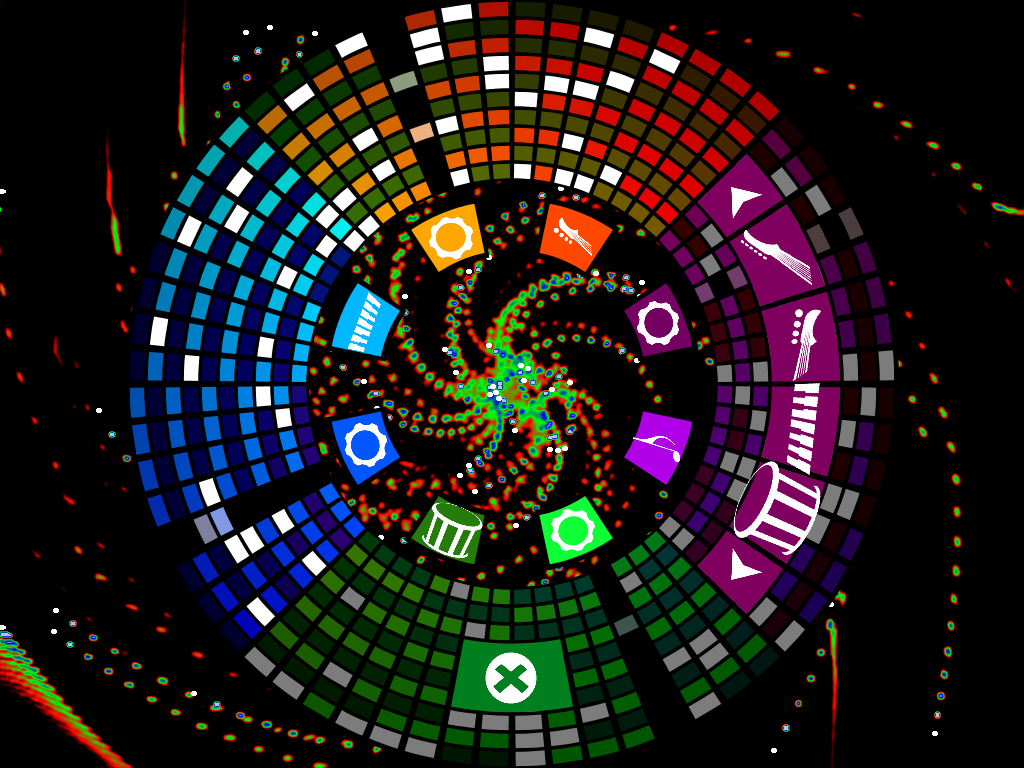
\includegraphics[width=84mm]{img/muziektafel_v3}
  \caption{Schets van het uiteindelijke ontwerp. Op het linker- en bovenste speelveld is de notenbalk met gecomponeerde melodie zichtbaar. Op het rechter speelveld is het instrumentkeuzemenu geopend. Op het onderste speelveld is de leegmaak-knop te zien. De spiraal op de achtergrond is de op de melodie gebaseerde visualisatie zichtbaar.}
  \label{fig:muziektafel_v3}
\end{figure}

Om te compenseren voor de verwijderde functionaliteiten is, ten behoeve van de langdurige speelbaarheid, wel besloten om meer dan vier instrumenten toe te voegen. Wanneer het instrumentkeuzemenu geopend is, kan met behulp van pijlen aan weerszijden van de instrumenten door de lijst met instrumenten gescrolled worden. Er is een piano, gitaar, basgitaar, saxofoon, drumstel, harp en triangel opgenomen. Om de functie van de instrumentkeuzeknop te verduidelijken, is het icoon hiervan vervangen door het instrument waarmee op dat moment gespeeld wordt. Wanneer het spel gestart wordt, gebruikt ieder speelveld standaard een verschillend instrument.

Tijdens de evaluatie van het LoFi-prototype kwam aan het licht dat niet iedereen de vier verschillend gekleurde gebieden identificeerde als losse speelvelden. De verwachting was echter dat dit kwam omdat het LoFi-prototype aan individuele proefpersonen is voorgelegd en niet aan groepen van twee of meer personen. In het uiteindelijke ontwerp is de keuze voor kleur als onderscheiding dan ook behouden. Wel is naar aanleiding van de LoFi-evaluatie besloten om de kwartmaten duidelijker te scheiden door de kleur van de rijen per vier noten om te draaien. Zie figuur~\ref{fig:muziektafel_v3}.

Vanwege technische moeilijkheden bleek de visualisatie zoals deze in de tweede iteratie van het ontwerp was opgenomen niet haalbaar. Er is daarom besloten tot een versimpeling van de visualisatie: iedere noot creëert een particle die met behulp van een visualisatie-library een draaiend en gekleurd effect krijgt.

Uit de LoFi-evaluatie bleek ook dat gebruikers niet begrepen hoe een geopend menu gesloten moest worden. Er is echter aangenomen dat deze onduidelijkheid veroorzaakt werd door de limitaties van een LoFi-evaluatie. Wanneer een gebruiker een menu opent en een keuze maakt binnen dat menu, zal het menu zich sluiten. Wanneer in het instrumentkeuzemenu een instrument gekozen wordt, sluit het zich en zodra in het instellingenmenu op de leegmaakknop geklikt wordt, sluit het instellingenmenu zich.

\subsection{Technisch Ontwerp}
\subsubsection{Datamodel}
De applicatie houdt een lijst met voor elke speler een tweedimensionale lijst van booleans bij van bepaalde lengte en hoogte. De lengte drukt tijd uit; booleans op dezelfde x-positie representeren tonen die simultaan afgespeeld worden, de hoogte bepaalt de toonhoogte. 

\begin{figure}
  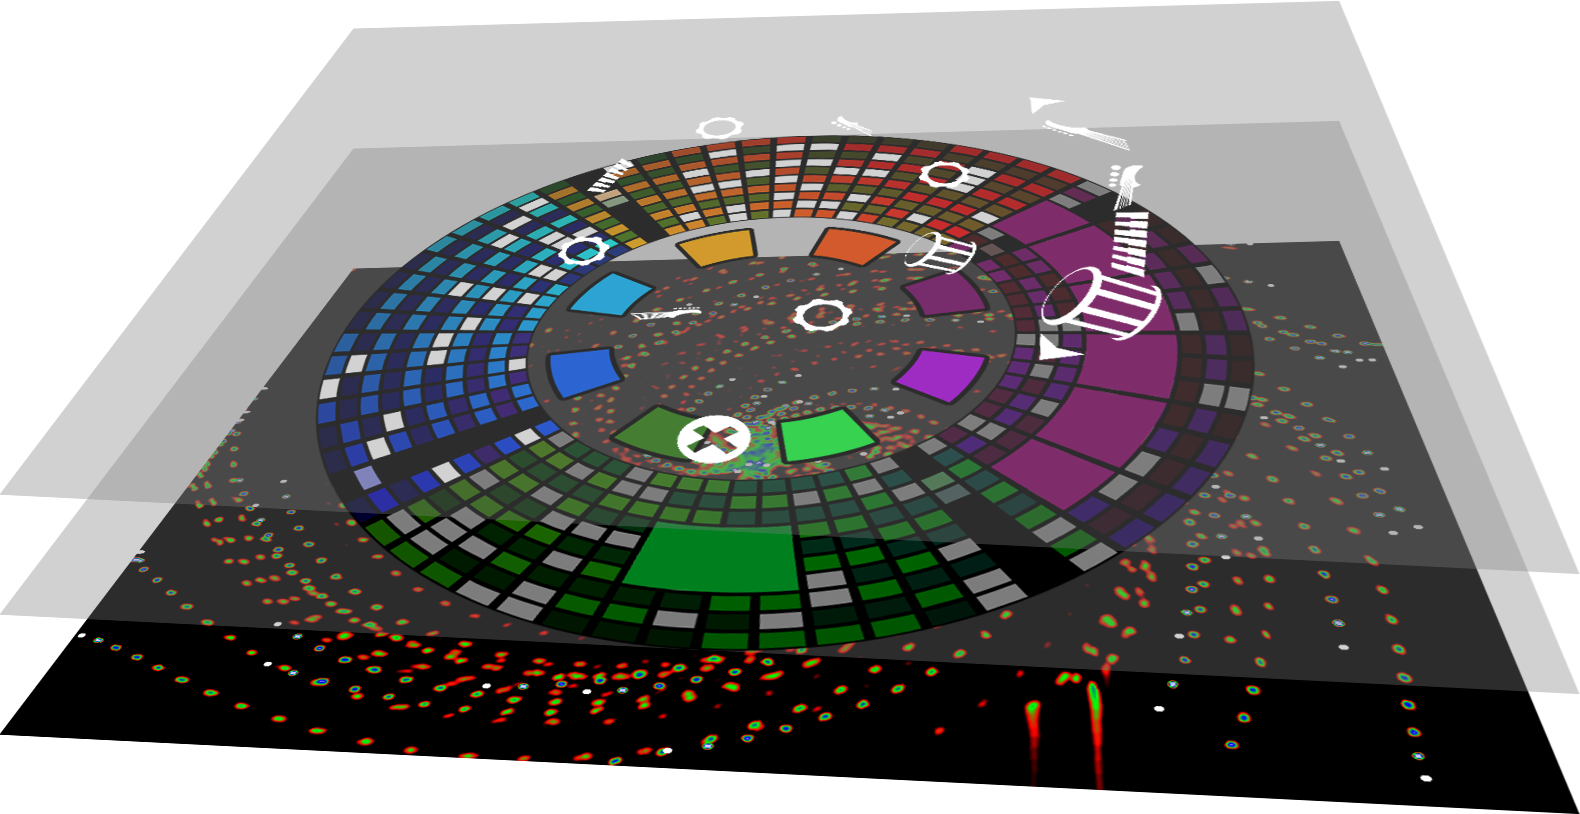
\includegraphics[width=84mm]{img/muziektafel_layers}
  \caption{Een visualisatie van de verschillende lagen in het ontwerp.}
  \label{fig:muziektafel_layers}
\end{figure}

\subsubsection{Datarepresentatie}
Deze spelergrids worden achter geplakt, en vervolgens omhoog gekromd tot de laatste weer aansluit bij de eerste, wat een donut-vorm oplevert. De waarde van elke boolean wordt vervolgens uitgedrukt in kleur; wit voor \textit{true} en een speler-specifieke kleur voor \textit{false}. De de kolommen die op een bepaald moment gespeeld worden, krijgen op dat moment andere kleuren; de spelerkleur voor \textit{true} en zwart voor \textit{false}. Hierdoor kunnen de spelers de tijdspositie van de muziek uitlezen.

\subsubsection{Interface}
De interface wordt gelaagd opgebouwd. Op de onderste laag wordt een visualisatie getekend op basis van de muziek die elk moment gespeeld wordt. Op de laag hierboven worden vlakjes getekend die de “muziekdonut” alsmede een aantal losse vlakjes die knoppen voorstellen. Op de derde laag worden iconen getekend, zoals een tandwiel voor het instellingmenu en het huidige gekozen instrument voor het instrumentmenu. Zie figuur~\ref{fig:muziektafel_layers} voor een visualisatie.

\subsubsection{Audio}
Voor de rendering van audio wordt de synthesizer uit \textit{javax.sound.midi} gebruikt.

\subsubsection{Visualisatie}
Wij maken gebruik van een externe library om de visualisatie te tekenen. De visualisatie genereert een particle voor elke noot die afgespeeld wordt. Vervolgens worden deze particles door een aantal filters getrokken om de visuele effecten te creëren.


\section{Evaluatie}
\label{sec_evaluatie}

\subsection{Opzet}
Voor de evaluatie van het HiFi-prototype is voor een eenvoudige aanpak gekozen. De proefpersonen is verteld dat ze met een multitouch-tafel gingen werken en dat ze zo lang mochten spelen totdat ze geen zin meer hadden. Eventuele vragen zouden niet beantwoord worden, maar als geconstateerd werd dat een proefpersoon echt niet wist wat hij of zij moest doen zouden ze op weg geholpen worden. Op deze manier wordt voorkomen dat een evaluatie verloren gaat als een gebruiker iets niet intuïtief begrijpt en kunnen aan de hand van overige observaties alsnog resultaten behaald worden.

De evaluaties zijn tweeledig opgezet: proefpersonen zijn geobserveerd terwijl ze met de muziektafel speelden en zijn achteraf verzocht een vragenlijst in te vullen. Om het intuïtieve karakter van de muziektafel te evalueren is bij de observaties gelet op de snelheid waarmee proefpersonen gebruik maakten van de beschikbare functionaliteiten. Gemeten zijn de tijd die het duurde voordat een proefpersoon een speelveld gekozen had, muzieknoten invoerde, van instrument wisselde en de leegmaakknop gebruikte. Ook werd bekeken of te zien was wanneer een gebruik klaar was met experimenteren en begon met het doelgericht componeren van een melodie. Naast deze kwantitatieve observaties, is ook bekeken hoe de proefpersoon zich gedroeg tijdens het werken met de muziektafel: had de proefpersoon plezier, was hij geïntrigeerd, communiceerde hij met de andere proefpersonen, hielp hij anderen of, wanneer er minder dan vier personen meededen, kwam de proefpersoon op het idee om meer dan een speelveld te gebruiken?

De enquête achteraf bestond uit een aantal kwalitatieve beoordelingen van bepaalde aspecten van de tafel en een aantal open vragen over hoe de proefpersoon het spelen met de muziektafel had ervaren en hoe de speler het samenwerken met anderen had ervaren.

De proefpersonen zijn ingedeeld in groepen van verschillende groottes, om te evalueren of de ontworpen muziektafel voor groepen van alle groottes een leuke ervaring is.

\subsection{Resultaten}
In totaal hebben 12 proefpersonen meegewerkt aan de eindevaluatie. Deze proefpersonen kwamen allemaal uit dezelfde leeftijdscategorie: tussen de 18 en 25 jaar. Drie van de proefpersonen waren vrouwen, de overige elf waren mannen. Twee proefpersonen hebben individueel met de tafel gewerkt en drie groepen van twee spelers en een groep van vier spelers hebben de muziektafel geprobeerd.

Het kiezen van een speelveld werd door de proefpersonen instinctief zonder oponthoud gedaan. Alleen de groep van vier spelers twijfelden kortstondig over welk persoon welk speelveld toebedeeld kreeg. Na onderling overleg was dit voor hen echter duidelijk en had iedereen een speelveld. Bij alle groepen van minder dan vier gebruikten de proefpersonen in eerste instantie alleen hun gekozen speelveld, maar wanneer ze tevreden waren over een gecreëerde melodie op hun eigen speelveld, weken ze al snel uit naar een aangrenzend speelveld om ook daar een melodie te maken. Toen bij een groep van twee een speler zich drie speelvelden had toegeëigend, werd hij door de andere speler hierop gewezen en stond hij er een af zodat ieder twee speelvelden had. Bij de groep van vier werd door de spelers ad hoc een competitief element bedacht, namelijk het zo snel mogelijk compleet vullen van de notenbalk, waarbij niet geschroomd werd andermans leegmaakknop te misbruiken door spelers om zelf het voordeel te krijgen.

Geen van de proefpersonen had na het kiezen van een speelveld moeite met het bedenken wat hij of zij moest doen: er werd meteen geklikt op de notenbalk of de instrumentkeuzeknop. Wel duurde het bij de meesten van hen even voordat ze doorhadden hoe hard ze moesten drukken om hun klik te laten registreren. Bij het bedenken wat er gedaan moest worden, maakte de groepsgrootte geen verschil, proefpersonen begonnen of meteen met het maken van een melodie of met het kiezen van een instrument om vervolgens een melodie te maken. Het instellingenmenu met de leegmaakknop werd gemiddeld pas na 2 minuten speeltijd ontdekt en gebruikt. Voor velen leek de ontdekking van die knop dat ook het moment te zijn waarop ze stopten met het willekeurig aanklikken van noten en begonnen met het doelgericht maken van een melodie.

Van de proefpersonen bracht het overgrote deel - 8 van de 12 - de tijd met de tafel vrolijk of lachend door, terwijl 2 van de 12 juist erg geconcentreerd bezig waren met het componeren van een melodie. Wanneer de bediening van de tafel het liet afweten, was bij alle proefpersonen enige frustratie waarneembaar, maar dat weerhield hen niet van doorgaan en alsnog vrolijkheid uitten tijdens de overige momenten van het spelen met de tafel. Bij een groep van twee proefpersonen leken beide proefpersonen niet erg geïnteresseerd te zijn gedurende het spel, maar zij gingen wel lang door met het spelen ervan. Uit hun enquêtes achteraf bleek dat ook zij plezier beleefd hadden aan de tafel, maar dat was niet zichtbaar in hun gedrag of gezichtsuitdrukking.

Alle proefpersonen bleef langer dan 5 minuten geboeid door de muziektafel. Vanwege de locatie van de muziektafel bij een bedrijf in productie, is gekozen om deelnemers na ongeveer 8 minuten te laten stoppen - waarna de meeste spelers ook aangaven dat het een mooi moment was om te stoppen. Vier van de 12 spelers vonden het oprecht jammer dat ze al moesten stoppen.

In de enquête gaf 11 van de 12 proefpersonen aan dat ze het spelen met de muziektafel leuk tot zeer leuk vonden, de overgebleven persoon vond het interessant. Wel werden bij deze beschrijving door 6 van de 12 proefpersonen meteen de kanttekening geplaatst dat een slechte calibratie en lage gevoeligheid van de muziektafel het speelplezier verminderd had.

De vraag wat ze het leukst vonden aan hun tijd met de speeltafel werd door 5 van de 12 beantwoord met het feit dat er muziek uit de tafel kwam en dat dat goed klonk. Vier van de 12 spelers vond het prettig dat de tafel simpel te bedienen en simpel te begrijpen was. Dit laatste werd ook duidelijk uit de vraag of spelers vonden dat ze de muziektafel eenvoudig te doorgronden was; 11 van de 12 spelers gaf aan dat dit het geval was. Als grootste gemiste features aan het programma werden een snelheidsregeling, een betere nauwkeurigheid en de kleine selectie instrumenten genoemd.

Op een schaal van 1 tot 5 werd de vindbaarheid van de notenbalk gemiddeld beoordeeld met een 4, de vindbaarheid van de instrumentkeuze met een 5 en de vindbaarheid van de leegmaakknop met een 3. De gebruikte instrumentengeluiden werden met een 3 beoordeeld, de animaties met een 4 en de gebruikte kleuren in het programma ook met een 4. Hardware-technisch kreeg de reactiesnelheid van de tafel een 4, terwijl de nauwkeurigheid een 2 kreeg. De zichtbaarheid van het scherm kreeg een 4, net als de grootte van de tafel. Het slepen werd met een 3 beoordeeld, maar sommigen ontdekten pas naar aanleiding van deze vraag dat het slepen mogelijk was.

Bij de groepen van meer dan 1 proefpersoon werd de samenwerking wisselvallend beoordeeld. Bij de kleinere groepen werd deze samenwerking positiever beoordeeld dan bij de groep van vier. De groep van vier gaf gemiddeld een 3 aan de samenwerking, terwijl de groepen van twee gemiddeld een 5 aan de samenwerking gaven. Deze trend was ook te zien bij de vraag hoe waardevol de spelers de samenwerking vonden voor het speelplezier. Bij de groep van vier gaf men aan dat iedereen zijn eigen ding deed of matig samenwerkte, terwijl men bij de groepen van twee juist aangaf dat de samenwerking een meerwaarde had. Het samenspel van de drukke melodieën bij de groep van vier spelers werd ook als negatief punt opgegeven. Wel gaven alle personen uit groepen aan dat de muziektafel niet zo leuk was geweest als iedere speler zijn eigen scherm had gehad. Het bij elkaar aan een tafel staan had een duidelijke meerwaarde. De proefpersonen die individueel met de tafel bezig geweest waren, gaven aan dat ze andere spelers niet tot nauwelijks gemist hadden.

\section{Discussie}
\label{sec_discussie}
De muziektafel is ontwikkeld om door meerdere mensen gebruikt te worden. Uit de evaluatie van individuele spelers bleek echter dat deze ook geschikt is voor enkele personen; zij kunnen genoeg uitdaging vinden in het componeren van een mooie melodie en het uitproberen van de verschillende instrumenten. Opvallend genoeg beviel de tafel voor de groep van 4 spelers minder dan voor de groepen van 2 spelers. De reden is waarschijnlijk de drukte die ontstaat als men vier drukke melodieën maakt die elkaar gaan overheersen. Door deze overheersing ging er snel anarchie heersen en werd een competitief element geïntroduceerd om de muziektafel alsnog leuk te krijgen. Van het oospronkelijke doel - muziek maken - was echter nog maar weinig over. Een enkele speler probeerde dit af en toe wel, maar werd overstemd door de rest, waardoor deze poging snel werd gestaakt. Een oplossing voor dit probleem is mogelijk het verminderen van het volume van een speelveld naarmate er meer noten zijn aangeklikt in dat speelveld. Op deze wijze kan worden voorkomen dat een speelveld de symfonie overheerst, waardoor de rest zijn speelplezier verliest.

Ondanks de wat mindere ervaring bij de groep met vier spelers werd de evaluatie ook door hen grotendeels lachend en vrolijk doorgebracht. Maar het lachen werd af en toe onderbroken door een frons wanneer de tafel het op technisch vlak liet afweten: de calibratie van de tafel kon als matig getypeerd worden. Naast de calibratie werd ook de tafel gevoeligheid van de tafel als negatief iets opgemerkt. Veel proefpersonen verwachtten dat een klik sneller geregistreerd zou worden en hadden pas na enige tijd door dat ze redelijk hard moesten drukken. Vermoedelijk is om die reden het slepen ook niet populair gebleken. Sommige proefpersonen ontdekten het slepen wel na een tijdje, maar maakten er alsnog niet heel veel gebruik van. De applicatie kan pas volledig tot zijn recht komen, wanneer de genoemde hardware-technische beperkingen opgelost zijn.

Wat positief verraste was de hoeveelheid tijd die proefpersonen wensten te spenderen aan het spelen met de tafel. De verwachting was dat spelers na vijf minuten wel genoeg zouden hebben van de tafel, maar alle proefpersonen speelden langer door en bleven experimenteren met nieuwe melodieën en andere instrumenten.


\section{Conclusie}
\label{sec_conclusie}
Er lag een generieke opdracht om een demo-applicatie te maken voor een multitouch-tafel; een applicatie die mensen moet uitnodigen tot het gebruik van de tafel. Na het doen van een aantal voorstellen aan de opdrachtgever is uiteindelijk de keuze gevallen op een muziektafel: een tafel waaraan meerdere personen tegelijk kunnen werken aan het componeren van een melodie op verschillende instrumenten. Toen er een initiëel ontwerp voor de interface lag, is door de projectgroep zelf geoordeeld dat deze niet zou kunnen voldoen aan de gestelde eis dat de interface intuïtief moest zijn. Na een herontwerp waar bepaalde functionaliteiten geschrapt zijn is het tweede ontwerp uiteindelijk als LoFi-prototype voorgelegd aan een groep proefpersonen.

De feedback hierop heeft geleid tot een aantal verdere verfijningen en verduidelijkingen in de interface. Een paar van de resultaten zijn echter toegeschreven aan het feit dat het LoFi-prototype niet interactief was en daarmee ook verminderd intuïtief. In het uiteindelijke ontwerp is opnieuw geschrapt in de beschikbare functionaliteit teneinde de intuïtiviteit te vergroten. Ook zijn de in het LoFi-prototype gevonden gebreken grotendeels verholpen.

Uit de evaluatie van het HiFi-prototype bleek dat de gedane aannames dat het juist was om te veronderstellen dat een interactief prototype intuïtiever zou zijn dan het LoFi-prototype; de onduidelijkheden die bij het LoFi-prototype genoemd zijn, zijn bij de eindevaluatie niet opnieuw gevonden. De muziektafel was intuïtief in het gebruik en het was voor de gebruikers een leuke ervaring om deze te gebruiken.

De groepsgrootte maakte wel uit voor de hoeveelheid lol die aan de muziektafel beleefd kon worden. Wanneer de groep groter dan twee personen werd, was er de neiging tot chaos. Hoewel deze chaos niet door iedere proefpersoon als negatief werd ervaren en leidde tot nieuwe manieren om de tafel te gebruiken, gingen hierdoor wel het doel van de applicatie en het daadwerkelijke gebruik ervan uit elkaar lopen: er werd door sommige spelers niet langer muziek gemaakt, maar juist gewerkt aan het zo snel mogelijk vullen van het speelveld.

Wat ook uit de eindevaluatie volgde, was dat de applicatie dient als echte demo-applicatie voor de tafel: het laat gebruikers kennismaken met zowel de positieve als de negatieve eigenschappen ervan. De hardware-technische beperkingen aan het registreren van kliks had een negatieve impact op het uiteindelijk speelplezier en de intuïtiviteit van de applicatie.

Desondanks was de respons tijdens de evaluatie overweldigend en werd getekend door het vele lachen en geïntrigeerd bezig zijn met het maken van muziek op een wijze die hiervoor niet mogelijk was. Hoewel er dus een aantal verbeterpunten zijn, kan gezegd worden dat een belangrijke eerste stap gezet is naar een nieuwe manier van coöperatief muziekmaken. En dat laat zien dat een multitouch-tafel een waardevolle toevoeging is op de steeds technischer samenleving.

\subsection{Future Works}
Uit de evaluatie zijn verschillende verbeterpunten komen rollen. Zo moet er onder andere gekeken worden naar het beter bruikbaarmaken van de applicatie wanneer er vier spelers zijn. Nu hebben de melodieën van de verschillende spelers de neiging elkaar te overheersen in plaats van elkaar aan te vullen. Wat hierbij ook zou helpen zijn realistischer geluiden voor de verschillende instrumenten. Momenteel wordt een MIDI-soundbank gebruikt, maar de uiteindelijke sympfonie is waarschijnlijk gebaat bij een betere samples van de verschillende instrumenten, die deze beter benaderen. Ook zou door het gebruik van dedicated samples per instrument het probleem verholpen worden dat verschillende machines momenteel verschillende MIDI-soundbanks bevatten en dat het opzoeken van de in de applicatie gebruikte instrumenten niet triviaal is; de instrumenten hebben in de verschillende soundbanks niet dezelfde naam, klinken verschillend en hebben een ander onderling volume.

Een leuke toepassing voor deze muziektafel zou zijn om deze te laten fungeren als MIDI-device waarmee de gecomponeerde melodie doorgestuurd kan worden naar professionele audio-software. Muziekproducers zouden op deze wijze de tafel kunnen gebruiken om net makkelijk, zo lang te tweaken aan hun melodie tot ze die melodie gevonden hebben die ze zoeken.

\section{Acknowledgments}
Tijdens dit project is door ons uitstekend samengewerkt met de medewerkers van KITT. In het bijzonder willen wij Mathijs van den Berg, Thomas van der Made en Andries Lohmeijer bedanken voor hun hulp en ondersteuning bij het koppelen van de applicatie met de multitouch-tafel en de nuttige feedback die zij gedurende het hele project hebben geuit.

\end{document}
